\def \methodname {TeAR\xspace}
\def \methodnamefull {Telemetry Assisted Racing\xspace}

\chapter{Design and Implementation}
This chapter provides a detailed description of the design and implementation of the software artefact employed in this project. The chapter starts by giving an overview of the core requirements for the main software artefact which we refer to as \emph{\methodnamefull (\methodname)} (see Section \S\ref{sec:imp-requirements}). Section \S\ref{sec:imp-content-creation} discusses the tools developed to create content for the feedback system, including track annotation and racing line visualisation amongst others. The chapter concludes with an in-depth description of the internals of the feedback system, the respective components, their integration and communication \ref{sec:imp-systemArchitecture}.

\section{Requirements}
\label{sec:imp-requirements}
Deliberation on the methodologies provided in Chapter \ref{chp:methodology} led to a number of requirements being identified for the software artefact. These requirements are listed below:

\begin{itemize}
	\item Content creation and annotation 
	\item Interfacing with third-party racing sim software 
	\item Efficiently read and process incoming telemetry stream
	\begin{itemize}
		\item Filter the stream for noise and unnecessary detail
		\item Structure raw data to facilitate further processing
	\end{itemize}
	\item Develop a heuristic-based system to provide feedback
	\item Provide a mechanism for communicating feedback to user
	\item Persist telemetry data for further processing
\end{itemize}

Circuit information coming from third-party software, such as the racing line, must be available to \methodname; furthermore, this data is to be annotated with additional information such as track section partitioning and the respective properties, which are fundamental in determining which feedback to provide to the user. Thus, a number of supporting tools have to be developed.
\methodname must interface with the third party racing simulation software (Assetto Corsa) via the inter-process communication system provided by the program. In addition, \methodname must extract a stream of telemetry data from the simulator, at a sampling rate of approximately 333Hz (which is the sustained rate provided by Assetto Corsa on the experiment's hardware).
The incoming telemetry data must be filtered since not all data is useful to \methodname. Furthermore, these data are organised into structures that are more conducive to processing later on in the pipeline. 
This telemetry information will be fed into a heuristic-based algorithm that should return feedback that will eventually be presented to the user. This feedback should be the most effective correction the user would need to make to improve that particular race track section.
\methodname should communicate this feedback to the user via an auditory messaging system. 
Finally, all telemetry data should be persisted onto secondary storage for offline analysis. 

\section{Content Creation and Annotation}
\label{sec:imp-content-creation}
The telemetry data stream read-out from Assetto Corsa does not provide sufficient information about the environment for \methodname to make informed decisions about possible feedback. The feedback mechanism used in \methodname is highly dependent on the racing line, which in turn, is a function of the track geometry; however, it is not possible to acquire any meaningful information about the racing track from telemetry data alone. These factors prompted the creation of the \emph{Track Splicer and Visualiser}, a supporting tool that extracts track information from the Assetto Corsa data files and provides additional annotations to this data as required by \methodname. 

\subsection{Track Splicing}
\label{sec:imp-trackSplicer}
The track splicing tool extracts track and racing line information from Assetto Corsa, partitions the data into a number of sections that are annotated as either straight or corner, and finally finds the apex of each corner section. The tool also provides visualisation of the results in case the user needs to tweak the generation parameters. This process is shown in Figure \ref{fig:diagram-trackspliceinputoutput}.

\begin{figure}[!htb]
	\centering
	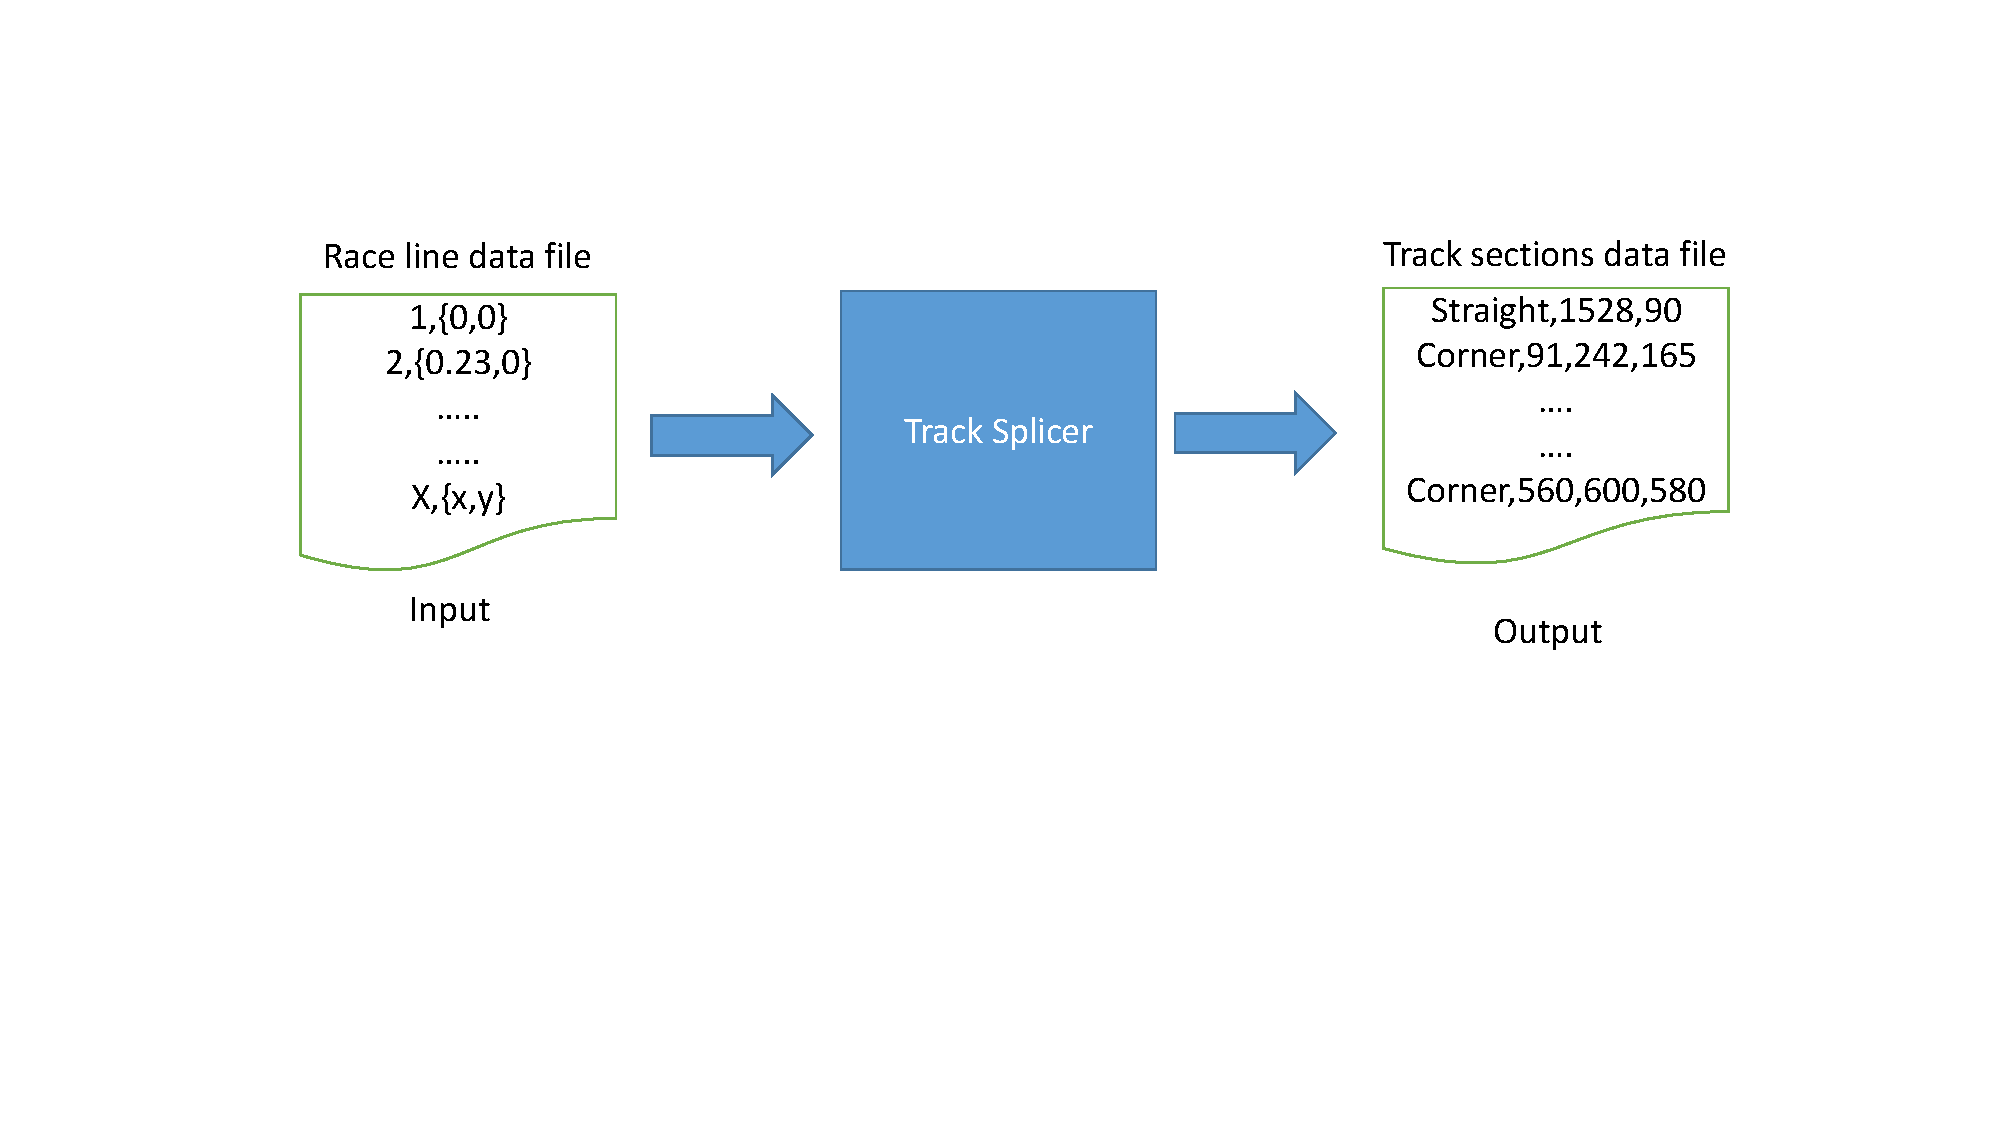
\includegraphics[width=\textwidth]{diagrams/trackspliceinputoutput.pdf}
	\caption[Track splicer input and out]{Track splicer input and output}
	\label{fig:diagram-trackspliceinputoutput}
\end{figure}

\begin{description}
	\item [Track Partitioning] The idealised racing line is a simple closed curve $\mathcal{C}$ on a plane; its digital counterpart is a discrete simple closed curve $\mathcal{C}_d$ with a finite number of vertices, each lying on the curve $\mathcal{C}$ and connected by straight edges - an inscribed polygon - where each vertex $\mathbf{v}_i \in \mathcal{C}_d$ represents a coordinate pair $(x,z)$. The ground is assumed to be a horizontal plane. 	To determine whether a section of the track near a vertex $\mathbf{v}_j \in \mathcal{C}_d$ is a straight or a corner, two further vertices are sampled $\mathbf{v}_i, \mathbf{v}_k \in \mathcal{C}_d$, where $i < j < k \in \mathbb{Z}/|\mathcal{C}_d|\mathbb{Z}$. We define the measure of curvature $c_j$ for the curve at $\mathbf{v}_j$ as follows:
	\begin{equation}
		c_j = \cos^{-1} \left(\frac{\mathbf{v}_k - \mathbf{v}_j}{|\mathbf{v}_k - \mathbf{v}_j|} \cdot \frac{\mathbf{v}_j - \mathbf{v}_i}{|\mathbf{v}_j - \mathbf{v}_i|} \right),
	\end{equation}
	where $c_j$ is the angle between the two normalised unit vectors formed by the ordered vertices $\mathbf{v}_i$ through $\mathbf{v}_k$. A threshold value $c_t$ determines whether the curve segment from $\mathbf{v}_i$ through $\mathbf{v}_k$ is a corner or a straight. A typical value for $c_t$ is 0.01. Edges between consecutive vertices in $\mathbf{C}_d$ may vary in length; therefore, when vertices $\mathbf{v}_i$ and $\mathbf{v}_j$ are chosen, Poisson-Disc sampling is employed, to guarantee that the vertices are no closer to each other than a specified minimum distance $c_m$ (a typical value for $c_m$ is 5).  	

	\begin{figure}[!htb]
		\centering
		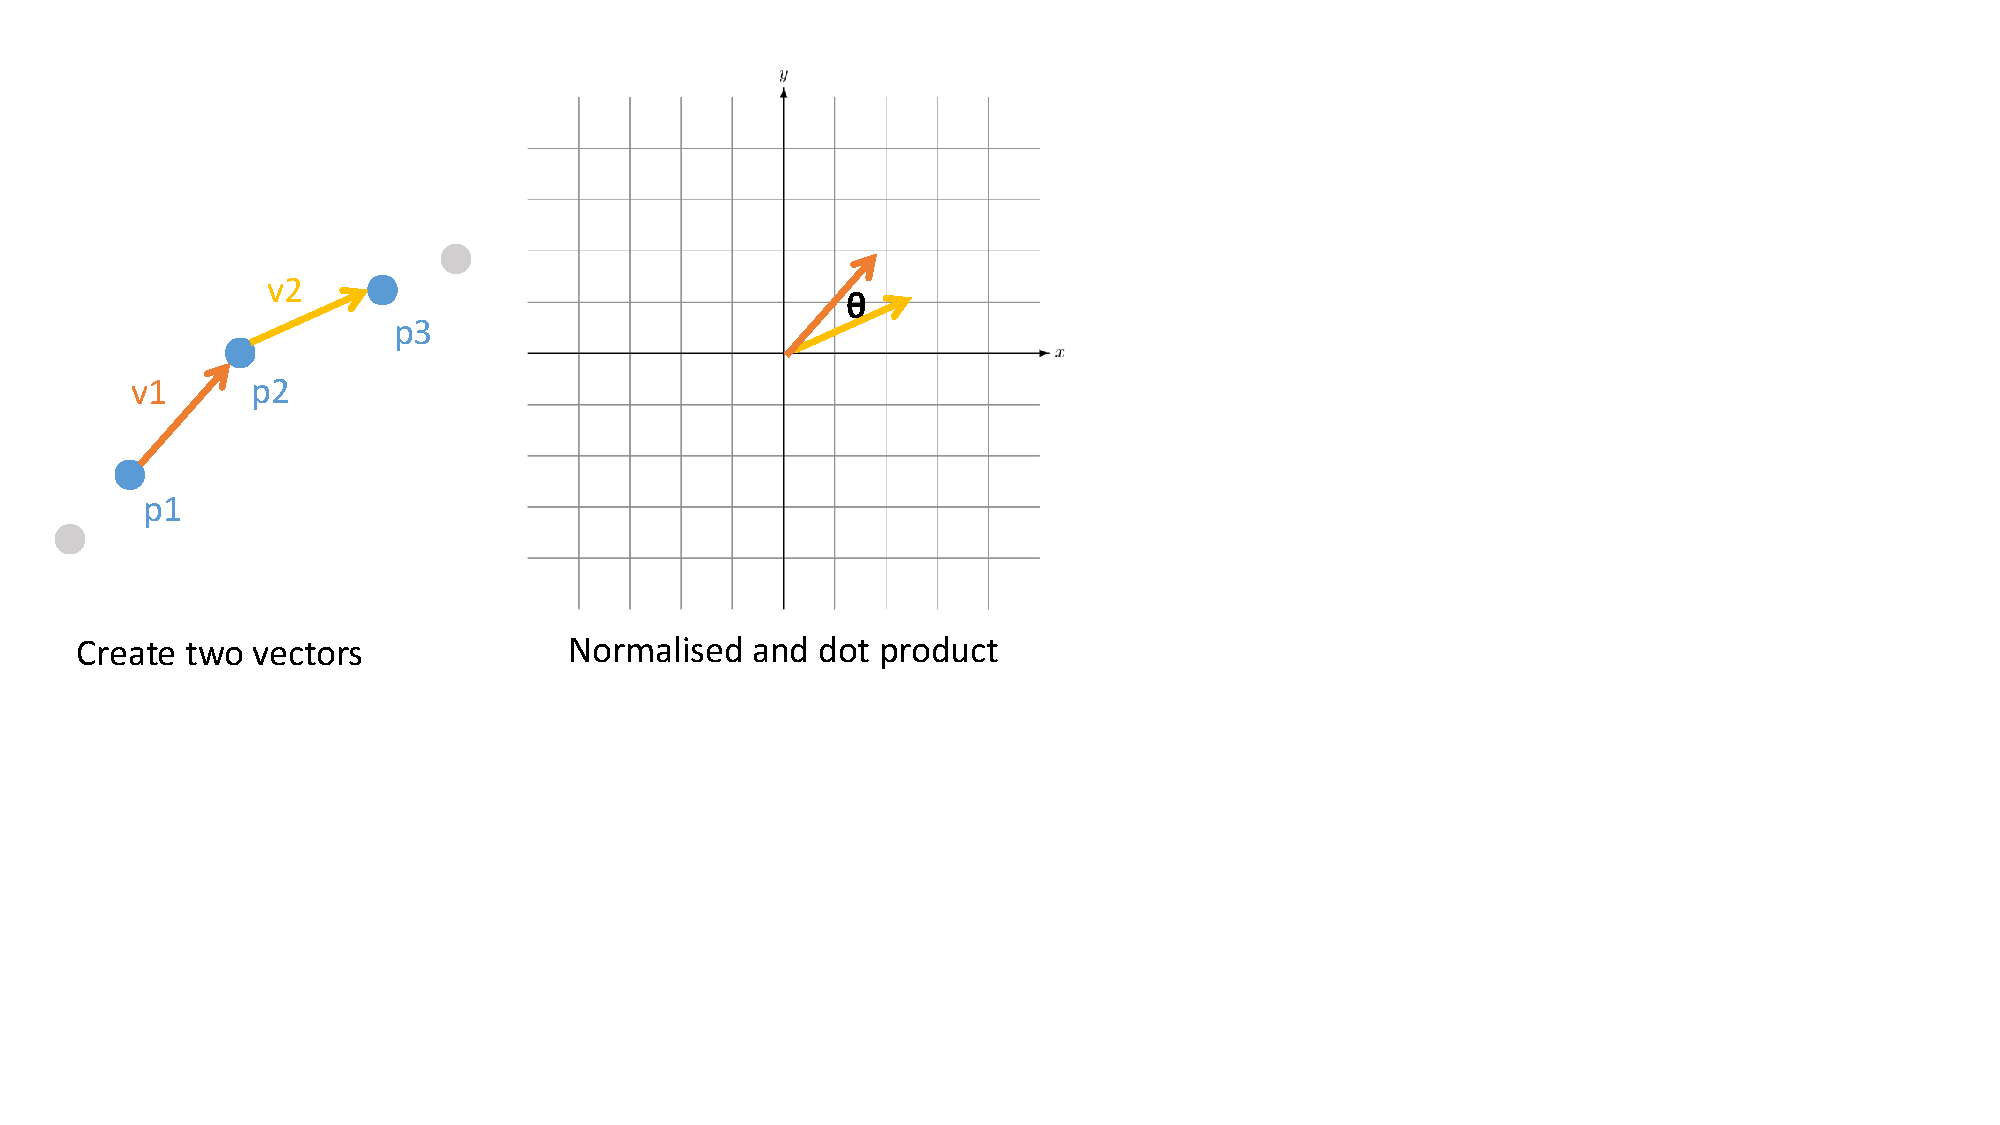
\includegraphics[width=\textwidth]{diagrams/vectorCorners.pdf}
		\caption[Splicing using vectors]{Points and vectors visualised}
		\label{fig:diagram-vectorCorners}
	\end{figure}
	
	\item [Track Annotation] The corner sections resulting from the partitioning process above are further annotated with the addition of the apex, or the corner midpoint vertex. The index $i$ of the midpoint vertex $\mathbf{v}_i$ is given by
	\begin{equation}
		\forall i,j | (\mathbf{v}_i - \mathbf{v}_0) \cdot (\mathbf{v}_{n-1} - \mathbf{v}_0)_{\perp} > (\mathbf{v}_j - \mathbf{v}_0) \cdot (\mathbf{v}_{n-1} - \mathbf{v}_0)_{\perp},  
	\end{equation} 
	where $0 \leq i,j < n$, for a corner section with $n$ vertices, and $\perp$ is the perpendicular operator such that $\mathbf{a} \cdot \mathbf{a}_{\perp} = 0$. 
	
	\begin{figure}[!htb]
		\centering
		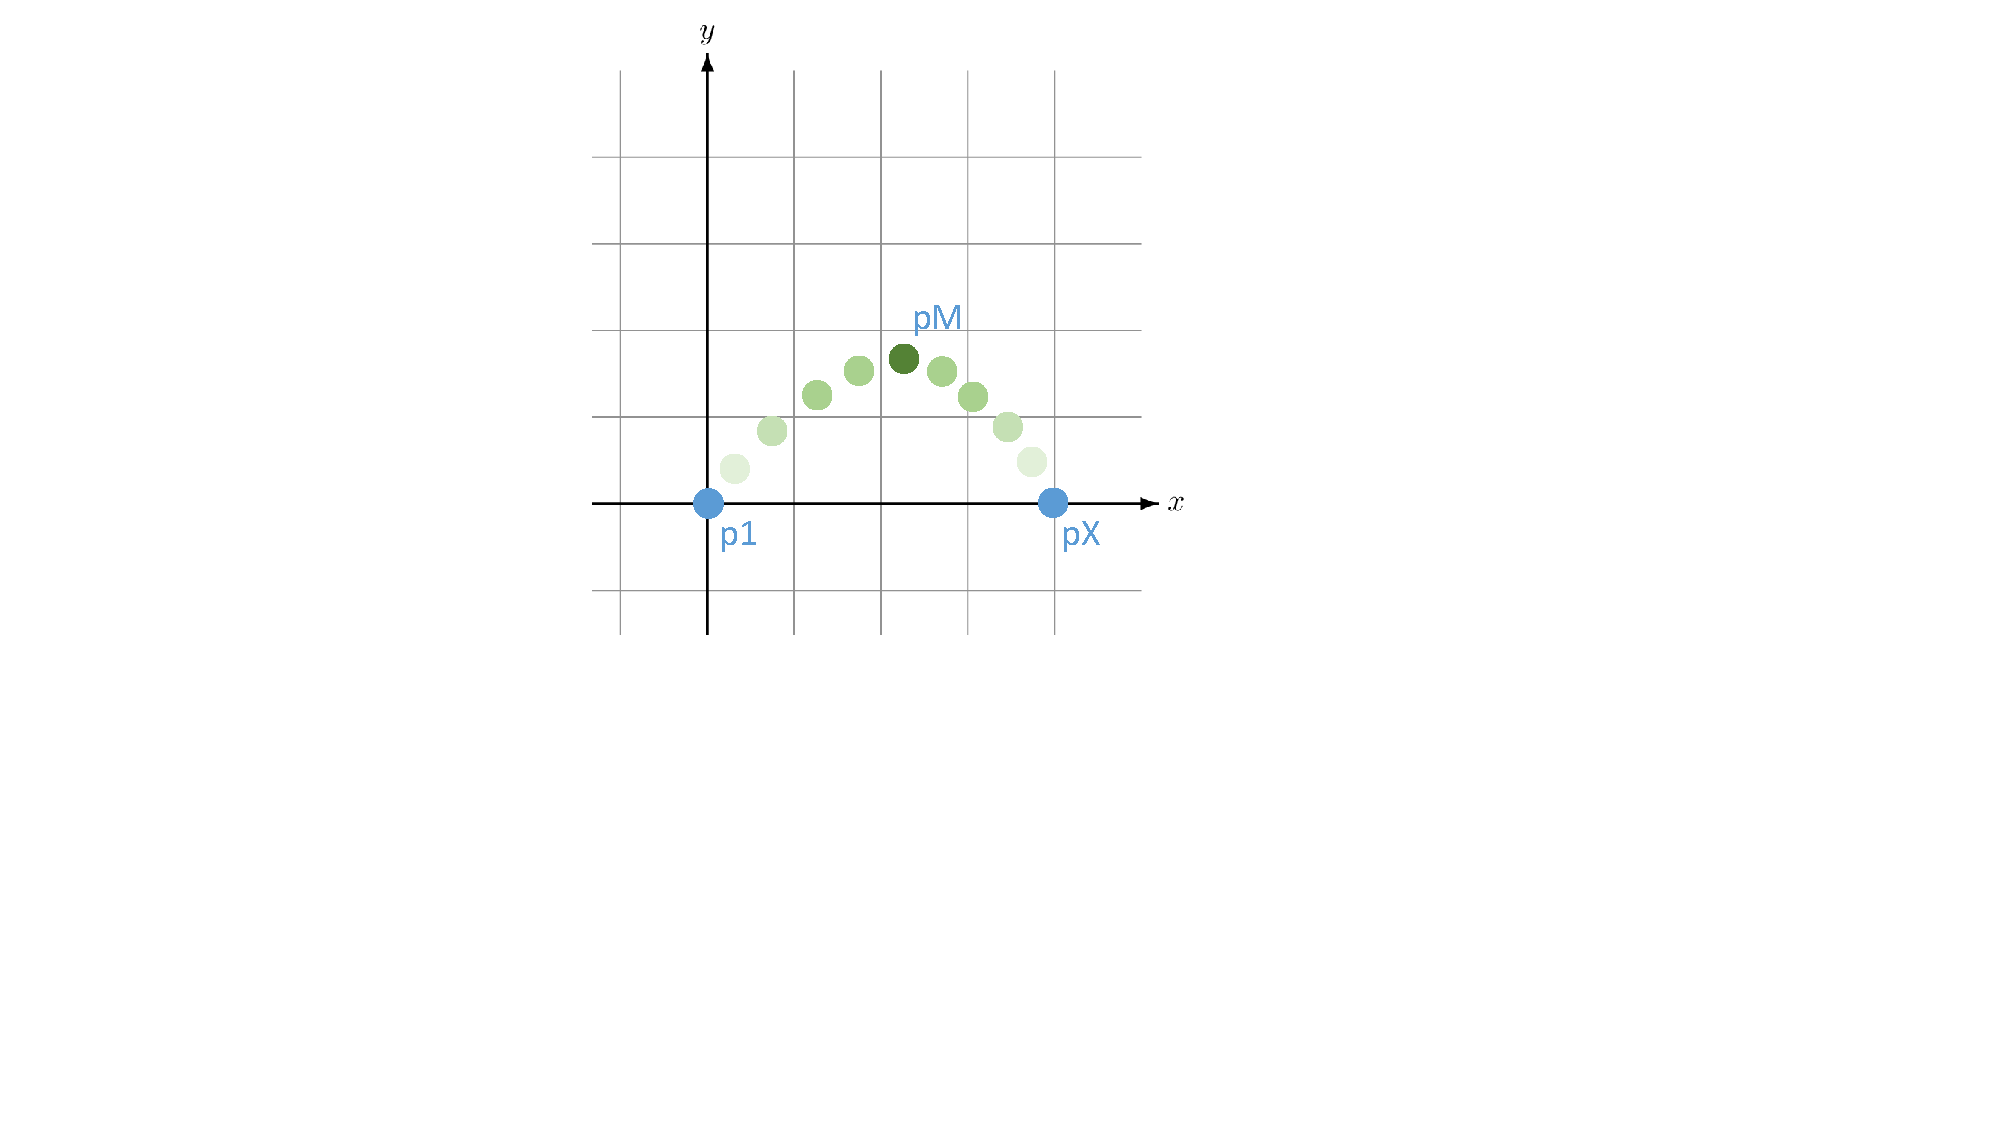
\includegraphics[height=5cm]{diagrams/cornerMidPoint.pdf}
		\caption[Corner mid point]{Finding the corner mid point}
		\textbf{p1} : First point \textbf{pM} : Corner mid point \textbf{pX} : Last point
		\label{fig:diagram-cornerMidPoint}
	\end{figure}
	
	\item [Visualisation and Tweaking] The partitioning and annotation of tracks is a semiautomated process; a visualisation component was added to the the track splicing tool, to display the partitioning results and bolster confidence in the transformed data. Furthermore, the visualisation helps in the tweaking of generation parameters ($c_m$, $c_t$, etc), by showing how changes in these values affect the output (see Figure \ref{fig:TrackSplicerTool}). 
	
	\begin{figure}[!htb]
		\centering
		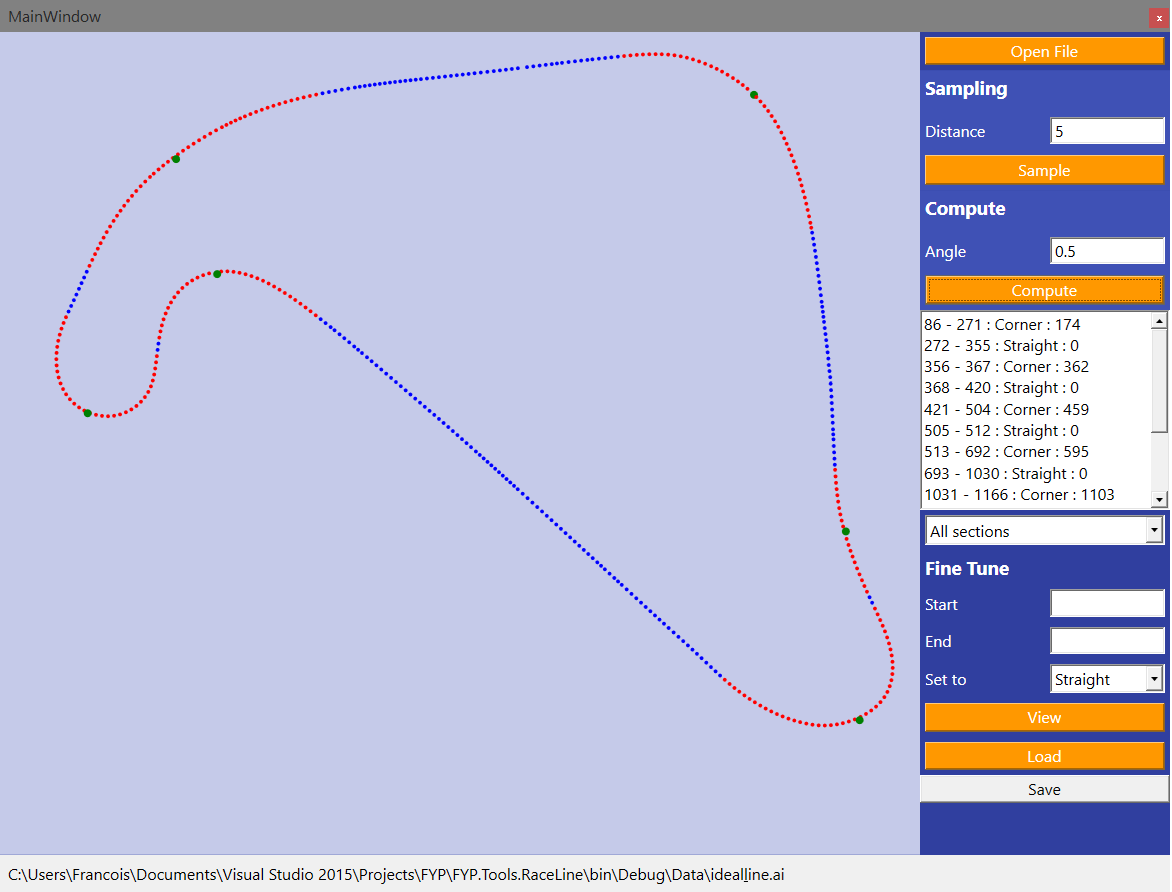
\includegraphics[height=5cm]{images/tracksplicertool}
		\caption{Track splicer tool}
		\textbf{Blue dots} : Part of a straight \textbf{Red dots} : Part of a corner \textbf{Green dots} : Corner mid point
		\label{fig:TrackSplicerTool}
	\end{figure}	
\end{description}

\subsection{Persistence of Telemetry Data}
Log files containing telemetry data from each user session are inserted into a database management system for offline analysis. An extraction transfer loading (ETL\cite{kimball2004data}) process (see Figure \ref{fig:ssis}) was purposely built, which takes as input a log file and inserts processed data as records into a database. This database is then used to run SQL queries related to the evaluation of the experiment.

\begin{figure}[!htb]
	\centering
	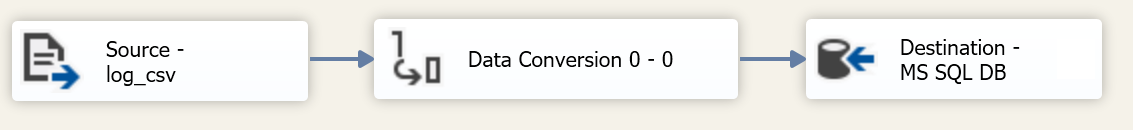
\includegraphics[width=\textwidth]{diagrams/ssis.png}
	\caption{ETL process using Microsoft's Integration Services}
	\label{fig:ssis}
\end{figure}

\subsection{Spatial Queries}
\label{sec:imp-SpatialQuerying}
In order for \methodname to determine the closest point on the racing line from the car's current position a spatial querying mechanism is required. Since TeAR provides real-time feedback on how the user is following the racing line, spatial queries are continuously carried out. Therefore, rather than using a linear search, a quad-tree data structure \cite{finkel1974quad} is used to store all the points on the racing line (see Figure \ref{fig:QuadTree}) and accelerate to $\mathcal{O}(\log{n})$ spatial queries. 

\begin{figure}[!htb]
	\centering
	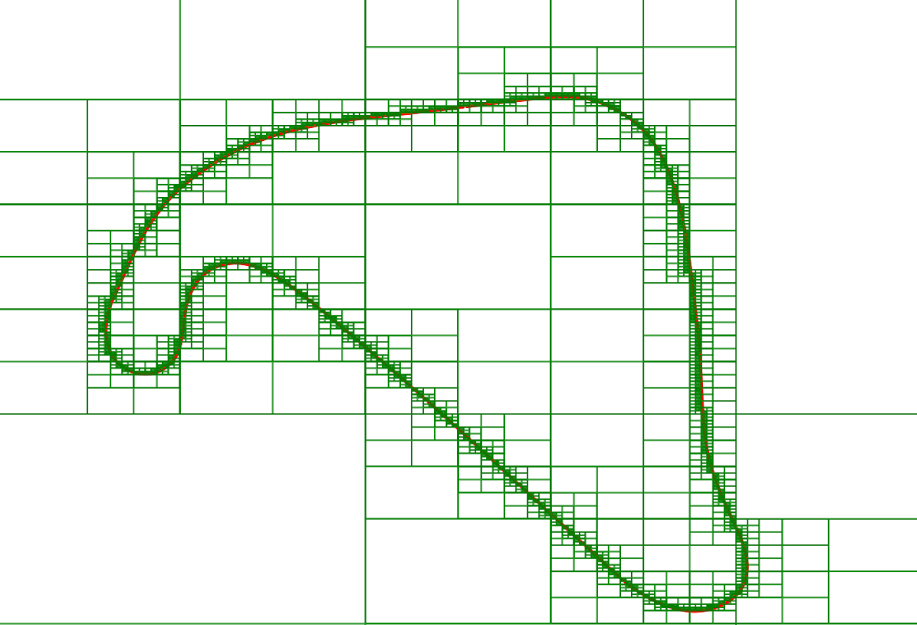
\includegraphics[height=5cm]{images/QuadTree}
	\caption{Visual representation for part of the quad tree for the Silverstone national circuit}
	\label{fig:QuadTree}
\end{figure}

\section{System Architecture}
\label{sec:imp-systemArchitecture}
\methodname is comprised of independent components which pass data to each other in order to select feedback instructions to be presented to the driver. Figure \ref{fig:SystemArch} illustrates the system architecture of \methodname. The following sections provide an in-depth overview of these components.

\begin{figure}[!htb]
	\centering
	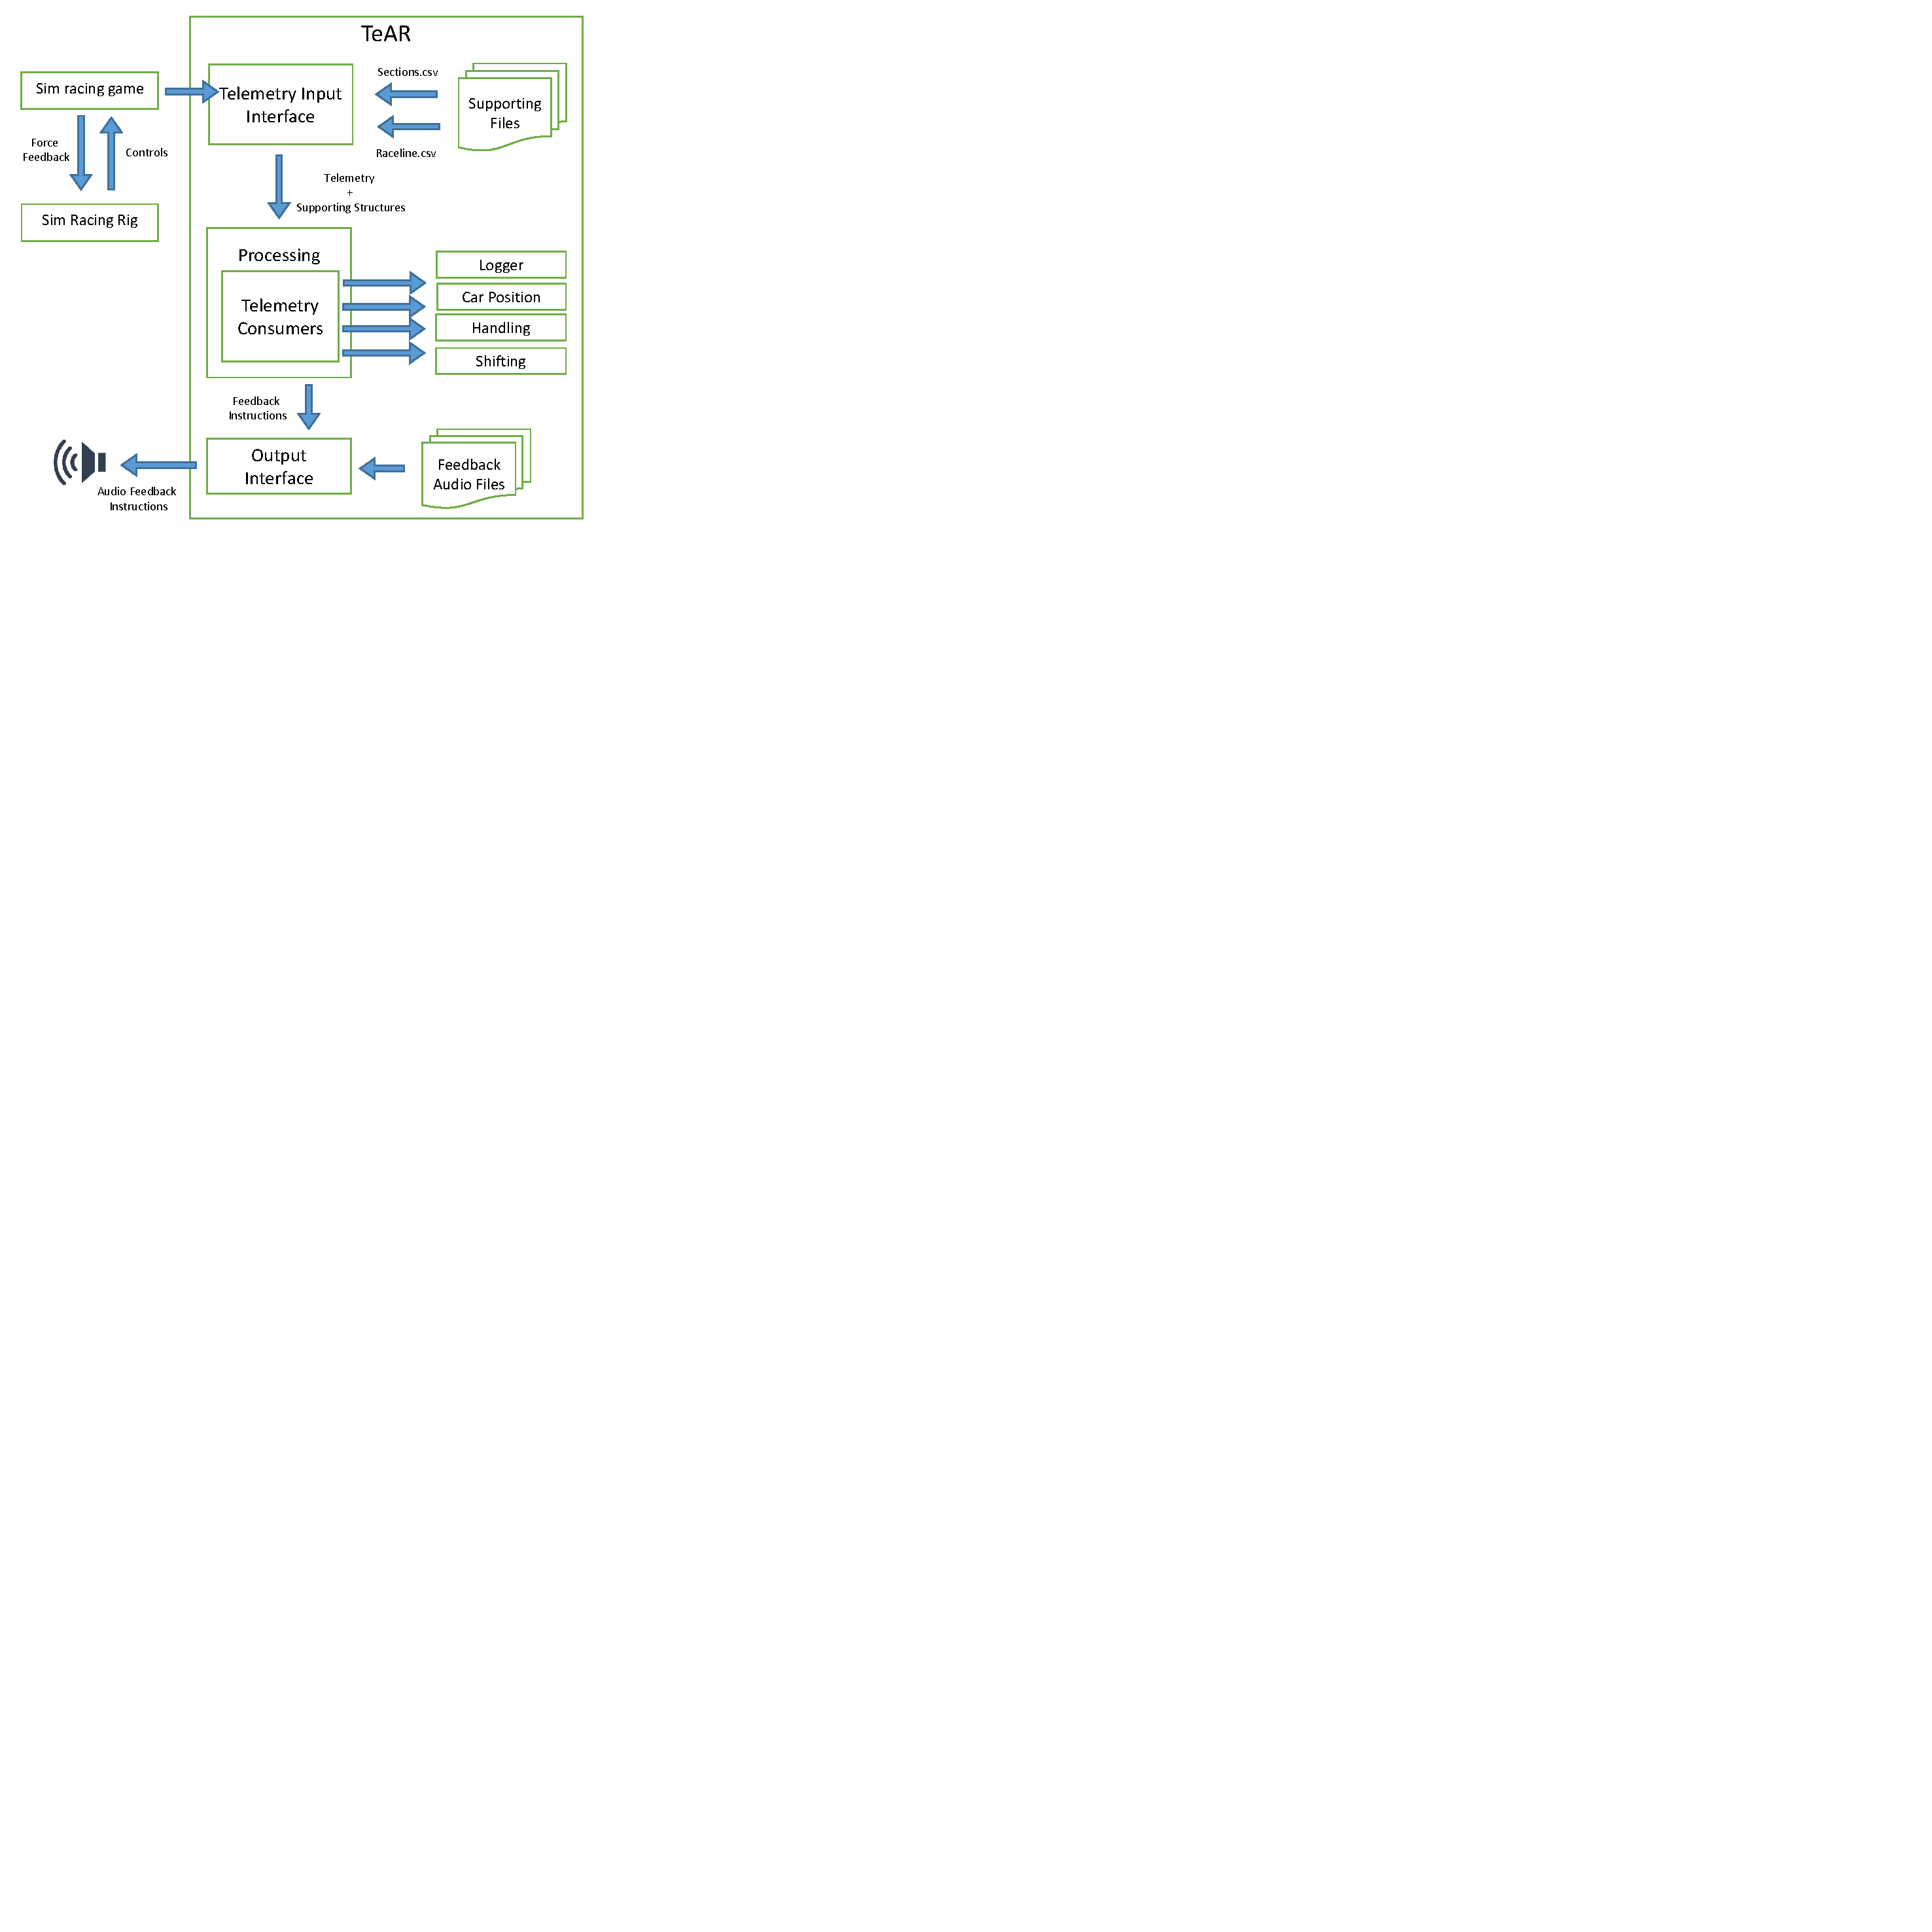
\includegraphics[height=10cm]{diagrams/SystemArch}
	\caption{Overview of the system architecture components}
	\label{fig:SystemArch}
\end{figure}

\subsection{Telemetry Input Interface}
This component handles all data input, either static on a per-track basis or real-time during a user's session. Static inputs include data generated by the track splicing tool. Real-time input is generated by Assetto Corsa which exposes a UDP server for \methodname to connect to and receive telemetry data.

\begin{figure}[!htb]
	\centering
	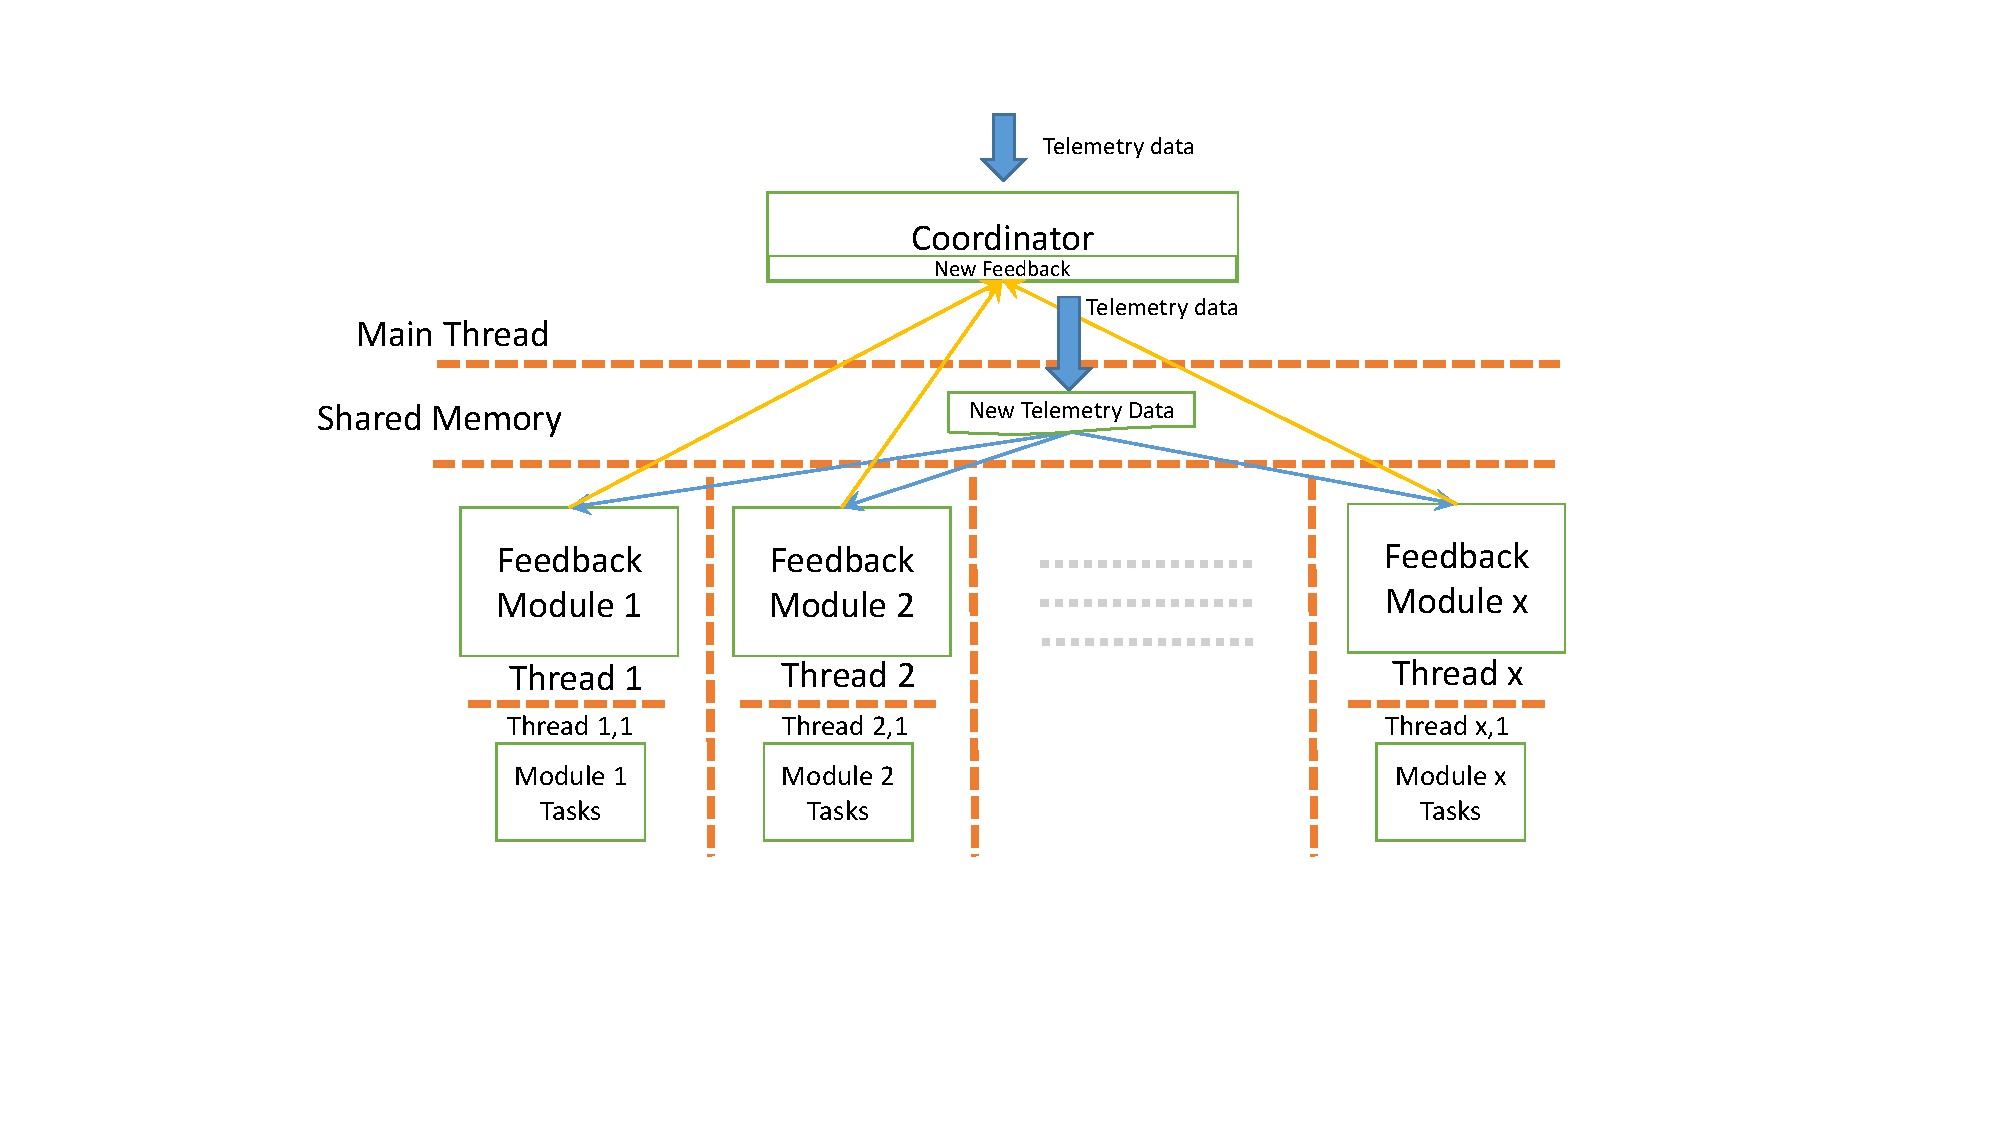
\includegraphics[width=\textwidth]{diagrams/multithreading.pdf}
	\caption{Overview of the coordination threading}
	\label{fig:multithreading}
\end{figure}

\subsection{Processing}
Telemetry data is consumed by the processing module, which coordinates a number of sub-modules each consuming the same telemetry data in a different way (e.g. Logger, Car Handling Feedback). These sub-modules run on separate threads and communicate and synchronise with the main processing module using shared memory. Any feedback notification raised by the sub-modules is captured by the processing module, which in turn forwards the message to the output module.

\subsubsection{Feedback Processing Sub-modules}
Although a number of sub-modules communicate with the processing module, to consume telemetry data, not all contribute towards the final user feedback that the system passes on to the output module. Those that contribute are termed feedback processing sub-modules and their collection comprises a static expert system. The rules and facts that make up this hand crafted expert system are derived from expert knowledge (see Chapter \ref{sec:background}).

The feedback processing sub-modules possess a common structure; each module is bound to a telemetry event. These events may be triggered by changes in one or more of the incoming telemetry data values. For example, while a braking event may be tied to a single telemetry datum, a gear-shift event requires examining data related to both the clutch pedal and the shifter. 

When an event is triggered, the respective sub-module will start the analysis process related to the respective telemetry information. Eventually, when the corresponding termination event (not necessarily tied to the same telemetry data as the activation event) is triggered, a decision is taken as to whether provide feedback or not, and if so, which feedback (see Figure \ref{fig:feedback-events}).

\begin{figure}[!htb]
	\centering
	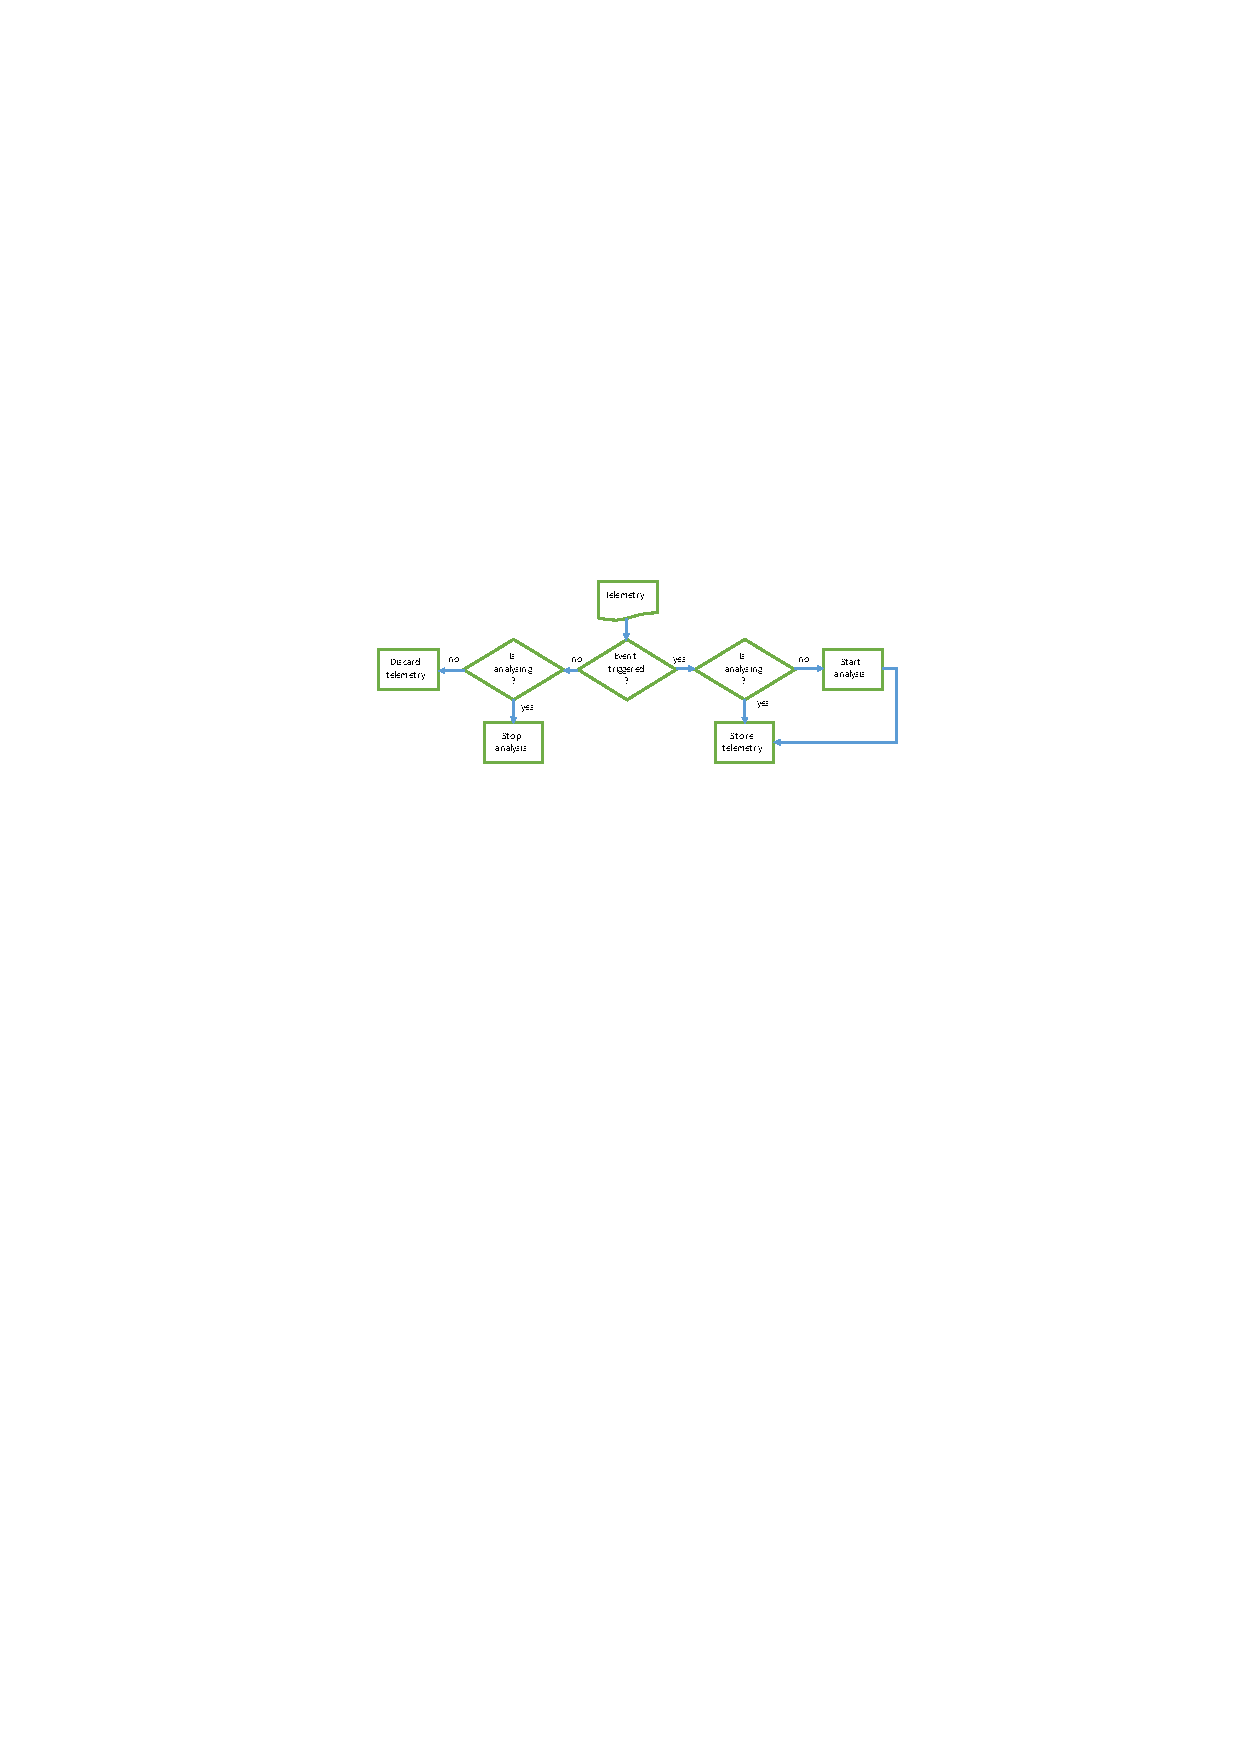
\includegraphics[width=\textwidth]{diagrams/feedbackEvent.pdf}
	\caption{Event triggering and stopping flow chart}
	\label{fig:feedback-events}
\end{figure}

The system operates using two feedback tiers; initially, at the first tier, only feedback related to the racing line is provided. As the user masters the racing line, the system will switch to the second tier and suggest more advanced feedback.

\subsection{Feedback Categories}
The feedback processing sub-modules each take care of a single skill category. Currently, three different categories are supported: (i) car handling, (ii) car positioning and (iii) gear shifting. 

\subsubsection{Car Handling}
This component monitors for braking and acceleration behaviours, and is able to raise the following feedback suggestions:
\begin{itemize}
	\item Braking too hard \\
	\begin{equation}
		slipratio_f > (15\% + tolerance_f)
	\end{equation}
	\item Braking too light
	\begin{equation}
		slipratio_f < (15\% + tolerance_f)
	\end{equation}
	\item Losing traction to the drive wheels by applying too much power
	\begin{equation}
		slipratio_r < -10\%
	\end{equation}
\end{itemize}

The rear and front $slipratio$ values are averaged over the period between the activation event and the termination event. The $tolerance_f$ value changes as the user improves; initially it is set to $7\%$ and have been determined through empirical observation.

\subsubsection{Car Positioning}
This component monitors for any divergence of the car from the racing line, and is able to raise the following feedback suggestions:
\begin{itemize}
	\item Braking in corner
	\begin{equation}
		braking * cornering > 0,
	\end{equation}
	where $braking$, $cornering \in {0,1}$; zero signifies false, one signifies true. 
	\item Incorrect race line during corner
	\begin{equation}
		cornering * dist > tolerance,
	\end{equation}
	where $cornering \in {0,1}$; zero denotes a straight segment, one a corner. $dist$ is the average car distance from the racing line for that section. $tolerance$ is initially set to 10, and is decreased as the user improves. The event triggers when the user transitions from a straight into a corner section ($cornering = 1$).
	\item Too aggressive during a corner
	\begin{equation}
		(cornering * slipangle_f) > 8\degree + tolerance,
	\end{equation}
	where $slipangle_f$ is the average slip angle for the front wheels.
	\item Too slow during a corner
	\begin{equation}
		(cornering * slipangle_f) < 8\degree - tolerance,
	\end{equation}
	where $slipangle_f$ is the average slip angle for the front wheels.
	
	Note that all averaged quantities are taken over the period between the activation event and the termination event.	
\end{itemize}

\subsubsection{Gear Shifting}
This component monitors for user gear changes, and is able to raise the following feedback suggestions:
\begin{itemize}
	\item Changing gear too soon
	\begin{equation}
		(8000 * (1 - shift_{up})) + rpm < 8000,
	\end{equation}
	where $shift_{up} \in {0,1}$; one denotes a gear change, and $rpm$ is the number of revolutions per minute of the car engine.	
	\item Changing gear too late
	\begin{equation}
		shift_{up} * rpm > 8500,
	\end{equation}
	where $shift_{up} \in {0,1}$; one denotes a gear change, and $rpm$ is the number of revolutions per minute of the car engine.
	\item Taking too long to transition from one gear to another
	\begin{equation}
		time_{neutral} > 0.5s
	\end{equation}
	where $time_{neutral}$ is the contiguous time spent in neutral gear position.
\end{itemize}

\subsection{Output Interface}
The final component in \methodname's pipeline is the Output Interface, through which feedback suggestions coming from the Processing module are presented to the user. This module connects to a repository of audio soundbites that map to the input feedback from the previous module. The audio files in the repository were generated using a free online text-to-speech tool \footnote{http://www.fromtexttospeech.com}. The module does not support concurrent playback of audio feedback by design, since this would overwhelm the user. Furthermore, since feedback is topical, buffering of feedback was intentionally omitted.

\subsection{Summary}
This chapter explained the requirements for \methodname and gave an explanation of the components which have been developed. Focus has been given to the inner workings on how feedback is generated. This is done by giving an explanation of each feedback's algorithm.